\chapter{Inference on Czech News sample}\label{inference}
A small experiment on czech news is provided. On sumeczech\footnote{\url{https://ufal.mff.cuni.cz/sumeczech}} \cite{straka2018sumeczech}



\section{Data}
popis dat, co ty columns obsahují, co naopak chybí. na kolika 

\section{Methodology}
text is splitted into sentences, labeled 0,1. The frequency is calulated -> article. Article-level features could be used (maybe conclusion). headline bias, also binary. Abstract bias. možná to uvest spíš jako: we measure bias on three levels. additionaly quoting bias.
Processing of domains: sport.novinky.cz -> novinky.cz


\section{Bias between domains}

\section{Bias along sections}
commentary wins

\section{quoting bias effects}
ctk vs denik

\section{Denik.cz}
on CTK there were only data in years 2016 and 2017. so no time plot

An example of classified news article can be seen in figure \ref{fig:demoarticle}. Note that 



\subsection{Application}
Additionally, I provide a simple web demo application for the reader to experiment with\footnote{\url{https://huggingface.co/spaces/horychtom/czech_media_bias_detection}}. The app runs on HuggingFace's spaces\footnote{\url{https://huggingface.co/spaces}} which is a free hosting service for demonstraing \gls{ml} applications. For the frontend, Gradio\footnote{\url{https://gradio.app/}} was used.

The user can insert arbitrary text in Czech language (text in other languages will result in meaningless outcomes). The text is then split into sentences and classified individually.

The app shows results in two output windows; first one \textit{classification} displays inserted text with highlighted labels. Second one, \textit{ratio}, displays ratio of biased/unbiased sentences in the text.

Example can be seen in \ref{fig:demodemo}.

\begin{figure}[h]
\makebox[\textwidth][c]{
  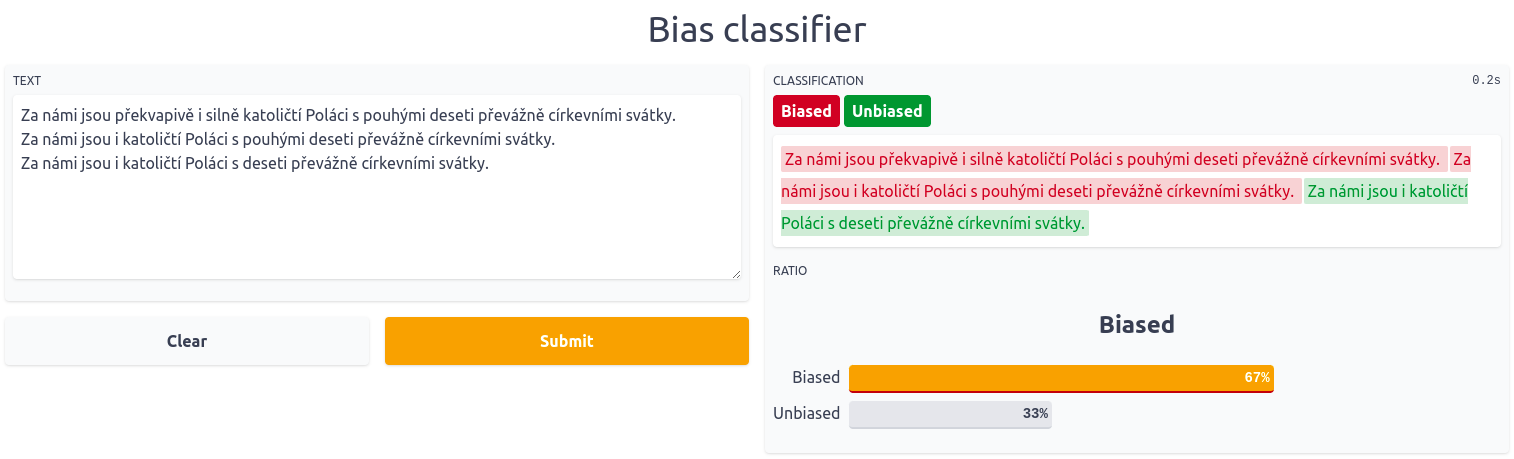
\includegraphics[scale=0.3]{my_modules/multimedia/bias.png}
  \caption{Example of the bias classifier demo usage.}
  \label{fig:demodemo}
  }
\end{figure}


\begin{figure}
\makebox[\textwidth][c]{
  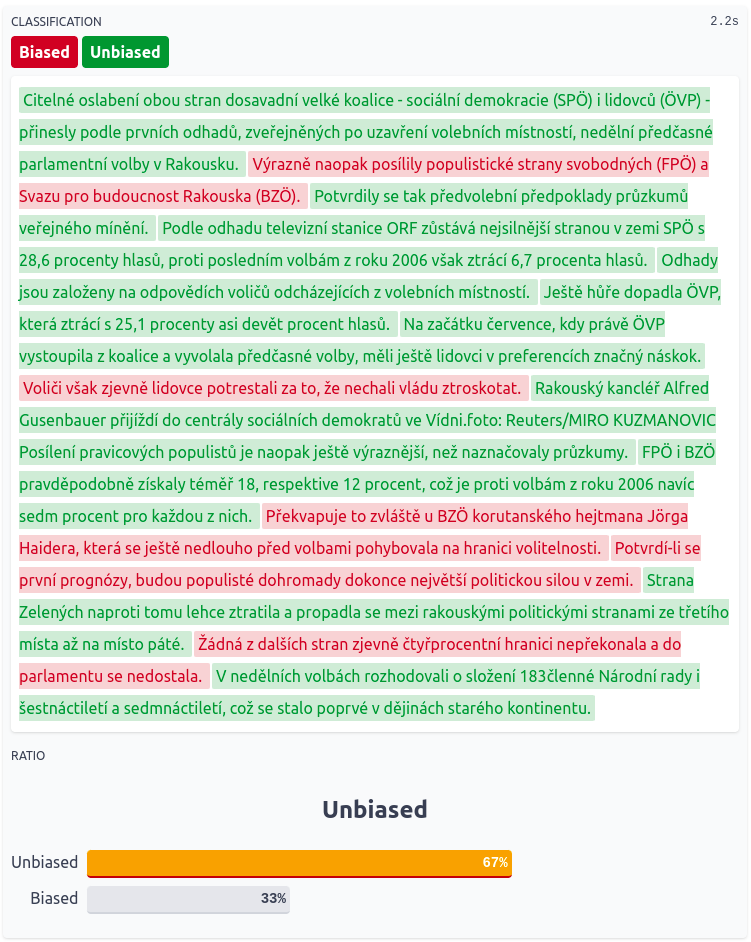
\includegraphics[scale=0.5]{my_modules/multimedia/article_example.png}
  \caption{Example of classified article.}
  \label{fig:demoarticle}
  }
\end{figure}

\section{Discussion}
Not all commentary articles are marked in the data.
Sometimes quoting is not marked, no discussion etc.
